% control regions, transfer factors
% binning in razor variables
% statistical treatment and systematic uncertainties


In light of the discussion in Section~\ref{sec:boost_motivation}, it is expected that boosted top
quarks are a promising signature of new physics involving a massive gluino decaying to a relatively
light top squark.
Boosted objects with high transverse momentum are characterized by merged decay products
separated by $ \Delta R \,{\sim}\, 2m/\pt$\footnote{Considering a heavy object $\W$ with mass $M$
that decays to two massless particles $a$ and $b$, we find $M^2 = 2 p_a \cdot p_b = 2 E_a E_b (1
- \cos{\theta_{ab}})$. Using the small angle approximation this becomes $M^2 = E_a E_b
\theta_{ab}^2$. Assigning half of the $\W$ energy to both $a$ and $b$ results in $M^2 =
\frac{1}{4} E_\W^2 \theta_{ab}^2$. Translating this relation into the transverse plane, we get
$\Delta R = \frac{2 M}{\pt^\W}$.}, 
where $m$ and $\pt$ denote the mass and transverse momentum of the mother particle, and $\Delta R$
is given in terms of azimuthal angle $\phi$ and pseudorapidity $\eta$ as $\Delta R = \sqrt{\Delta
\phi^2 + \Delta \eta^2}$.
For a separation of $\Delta R = 0.5$, the standard cone size of jets used in CMS, a top
quark should thus have a momentum of ${\sim}700$\GeV, a value difficult to reach with proton-proton
collisions at 8 TeV. 
Therefore, in order to increase the signal efficiency, we consider instead $\W$ bosons from top
quark decays, which are required to have a more accessible $\pt \,{\sim}\, 320$\GeV.  This results
in an increase in the signal efficiency of a factor of about 3--5, depending on the mass
spectrum considered. 
Targeting $\W$ bosons instead of top quarks also allows us to use smaller cone sizes, resulting in
jets with smaller uncertainties.
The \pt of the top quark and $\W$ boson at the generator
level without applying any selection, is shown in Figs.~\ref{fig:boost_gen_toppt} and
\ref{fig:boost_gen_Wpt} for several signal models, and the SM $t\bar{t}$ process. 
We observe that the average \pt is higher for the signal than for $t\bar{t}$. Requiring the
presence of a boosted $\W$ boson will thus be part of the strategy to reduce the SM background.
Hadronically decaying boosted $\W$ boson candidates will be identified using pruned jet
mass~\cite{Ellis:2009su,Ellis:2009me,Chatrchyan:2013vbb} and a jet substructure observable
called N-subjettiness \cite{Thaler:2010tr}. Full details on the $\W$ tagging technique will be given
in Section~\ref{sec:boost_wtag}. 

\begin{figure}[htpb]
\centering
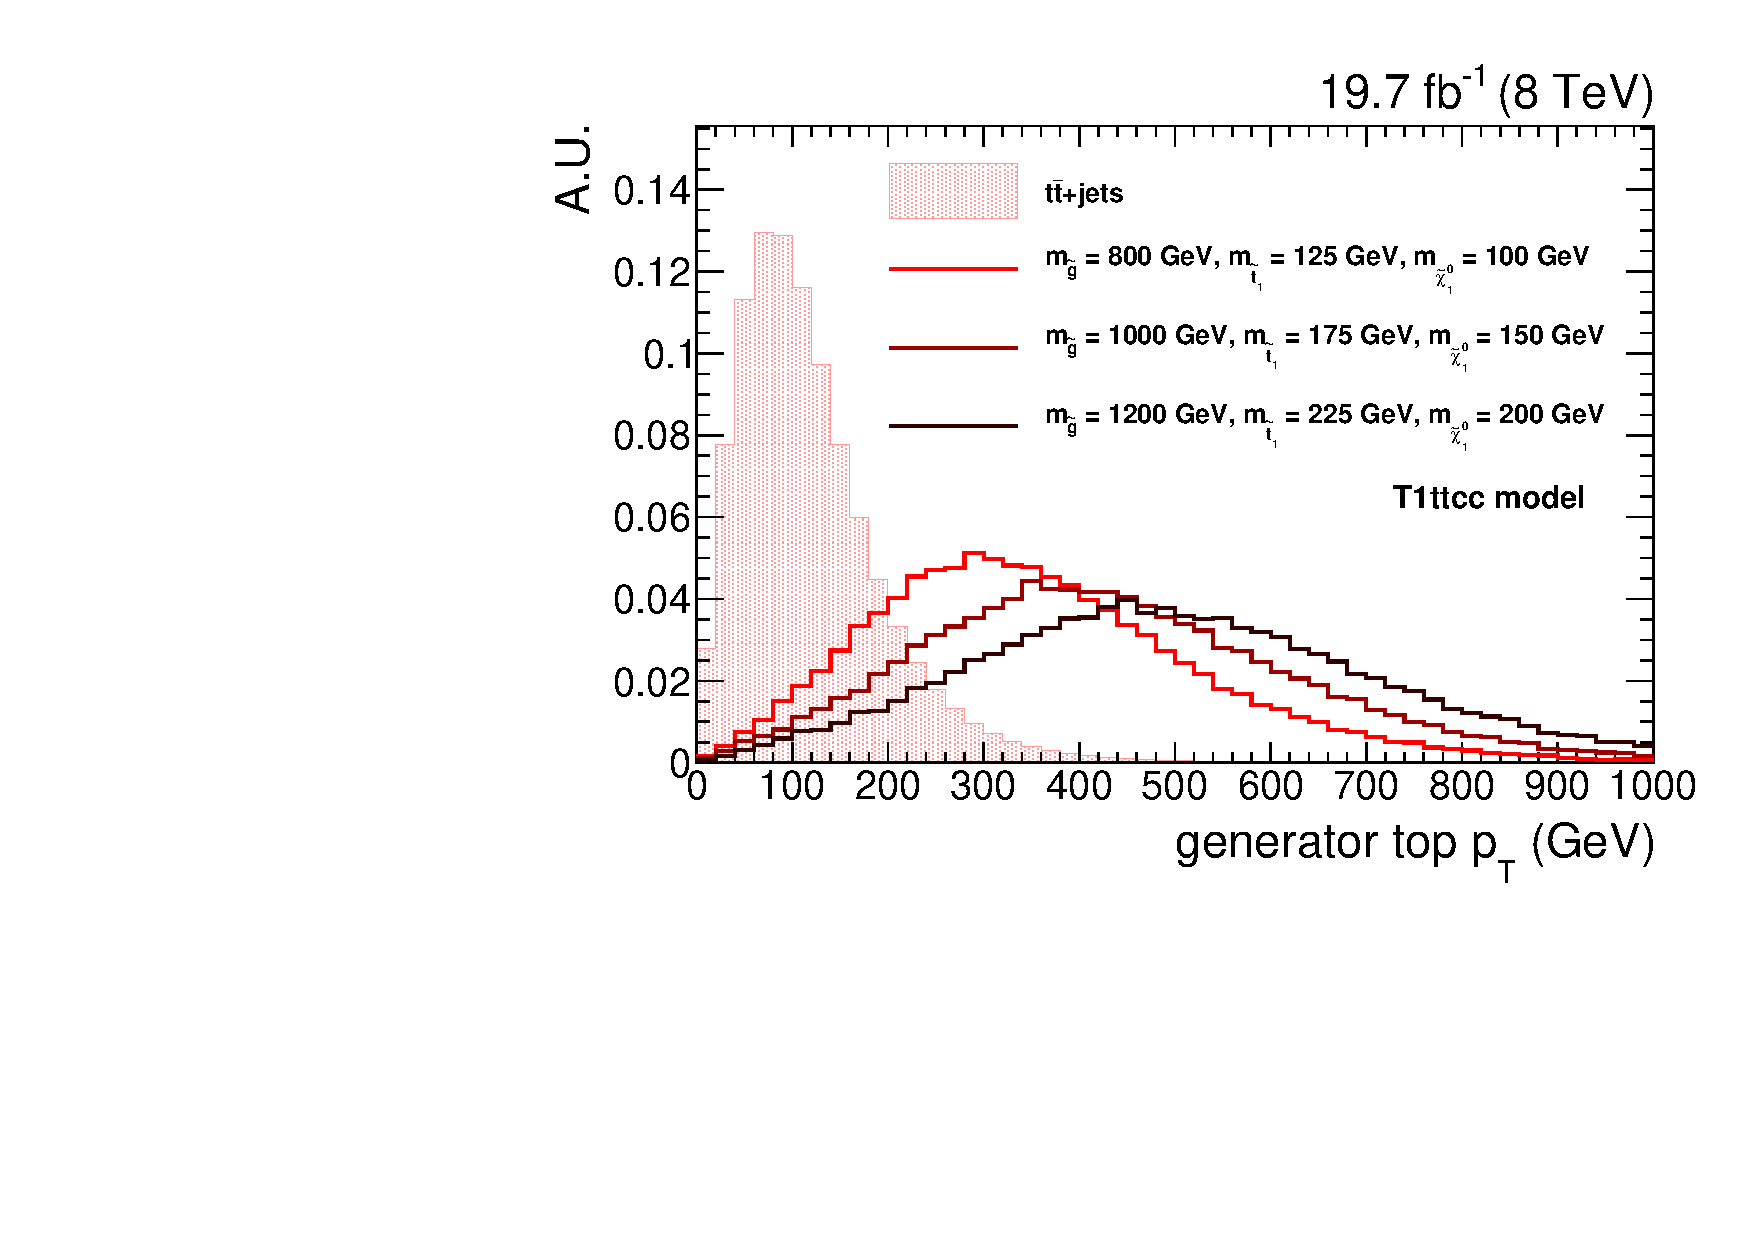
\includegraphics[width=0.48\textwidth]{figures/razor_strategy/T1ttcc_gentoppt}
~
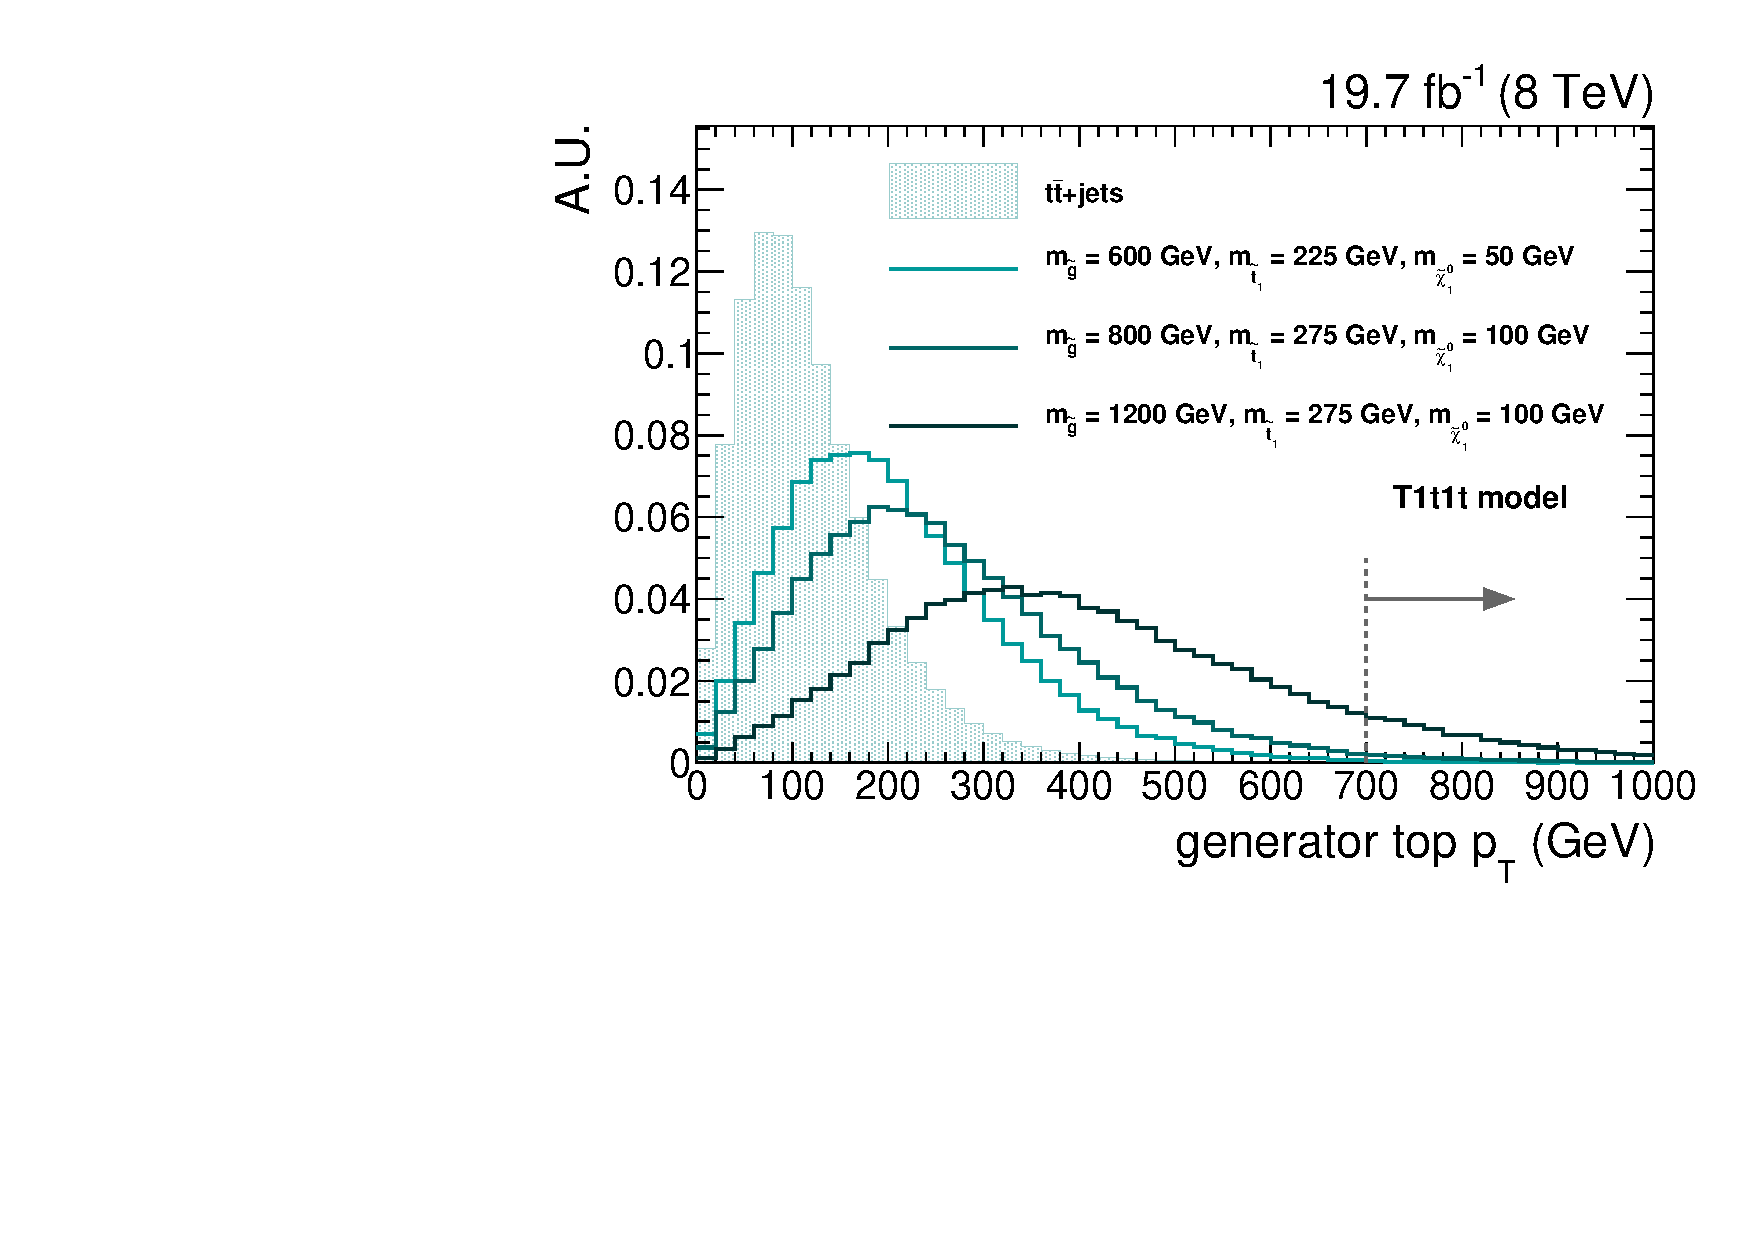
\includegraphics[width=0.48\textwidth]{figures/razor_strategy/T1t1t_gentoppt}
\caption{Generator level top quark \pt for several signal points of the T1ttcc (left) and T1t1t
(right) simplified models. The average \pt increases as the mass splitting between gluino
and top squark increases. The boost of
the top quark is larger for the signal models considered in comparison to the SM $t\bar{t}$
background. 
The range in \pt needed to have merged decay products for jets with size $\Delta R = 0.5$ is
indicated with an arrow. 
\label{fig:boost_gen_toppt}}
\end{figure}
\begin{figure}[htpb]
\centering
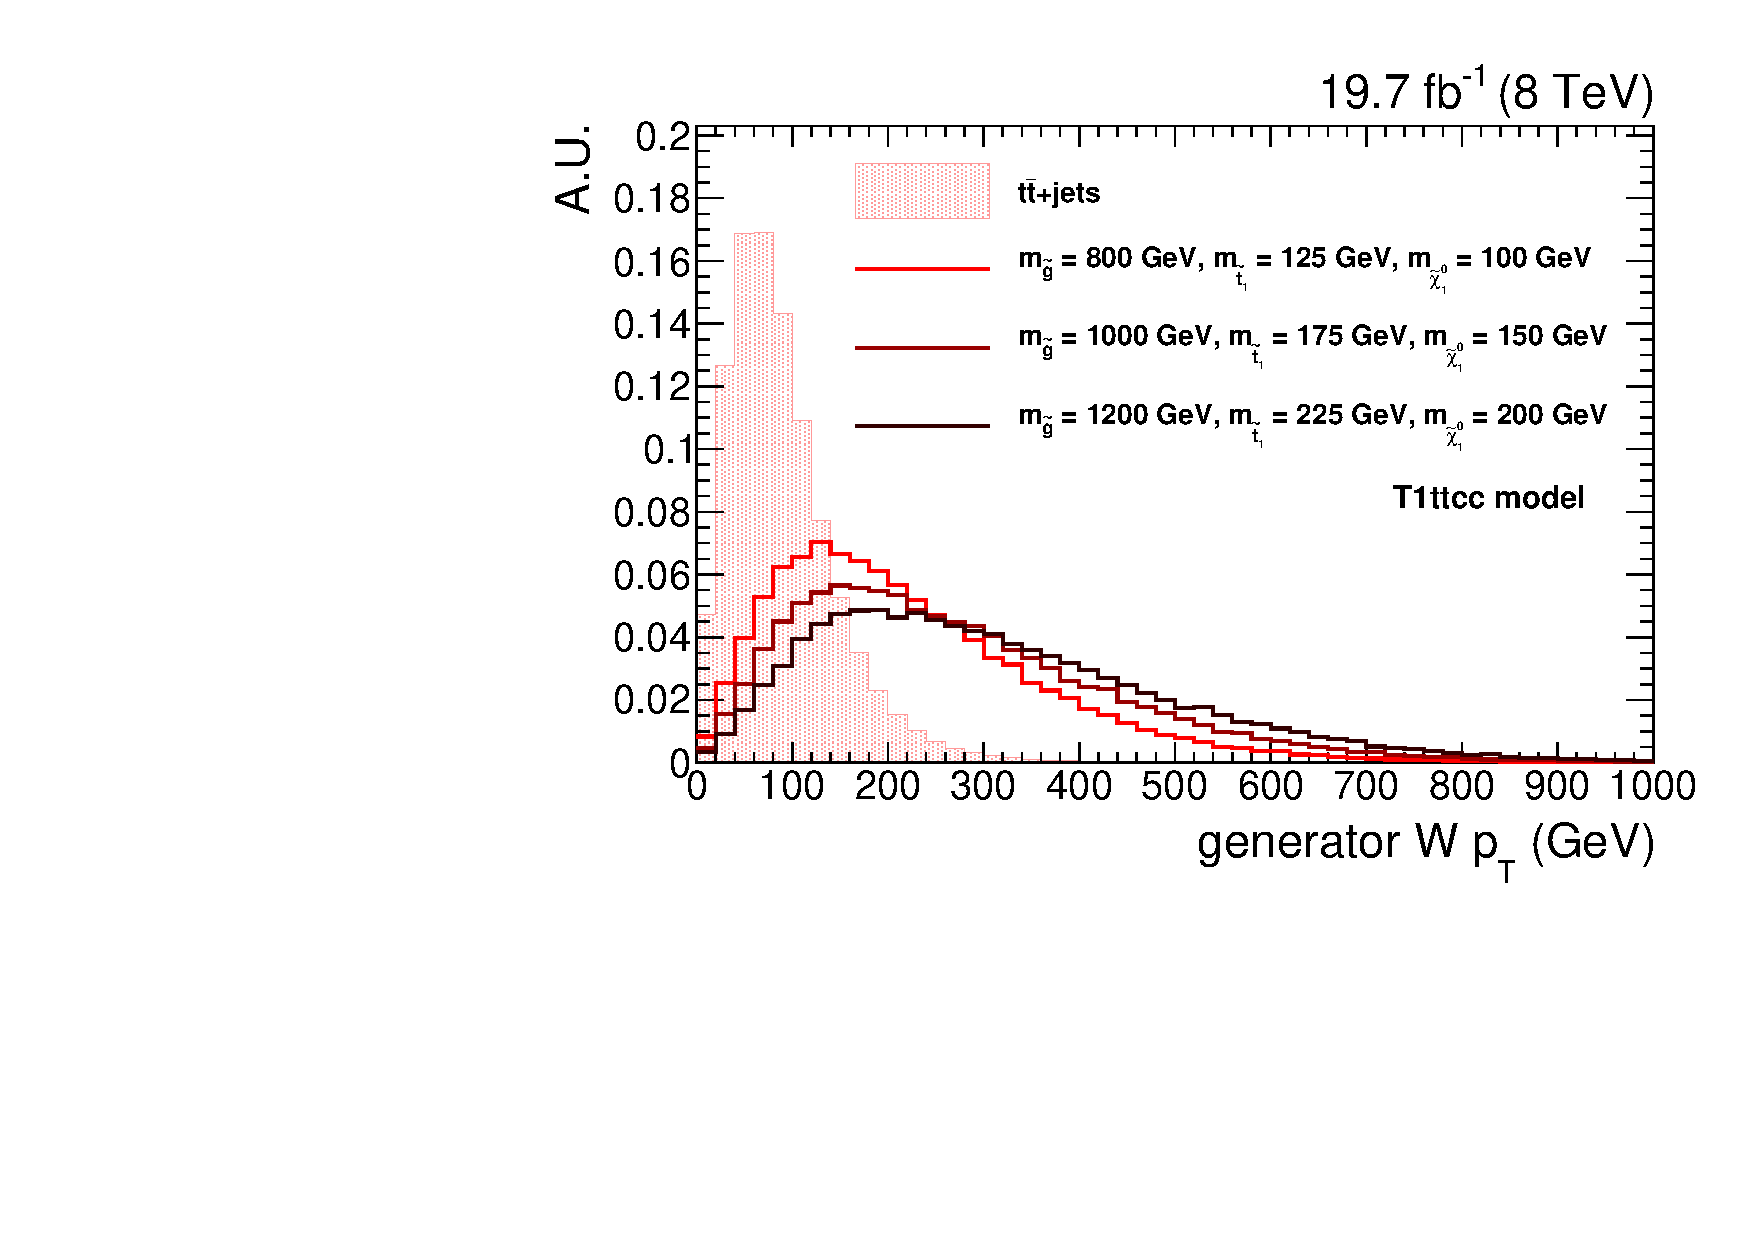
\includegraphics[width=0.48\textwidth]{figures/razor_strategy/T1ttcc_genWpt}
~
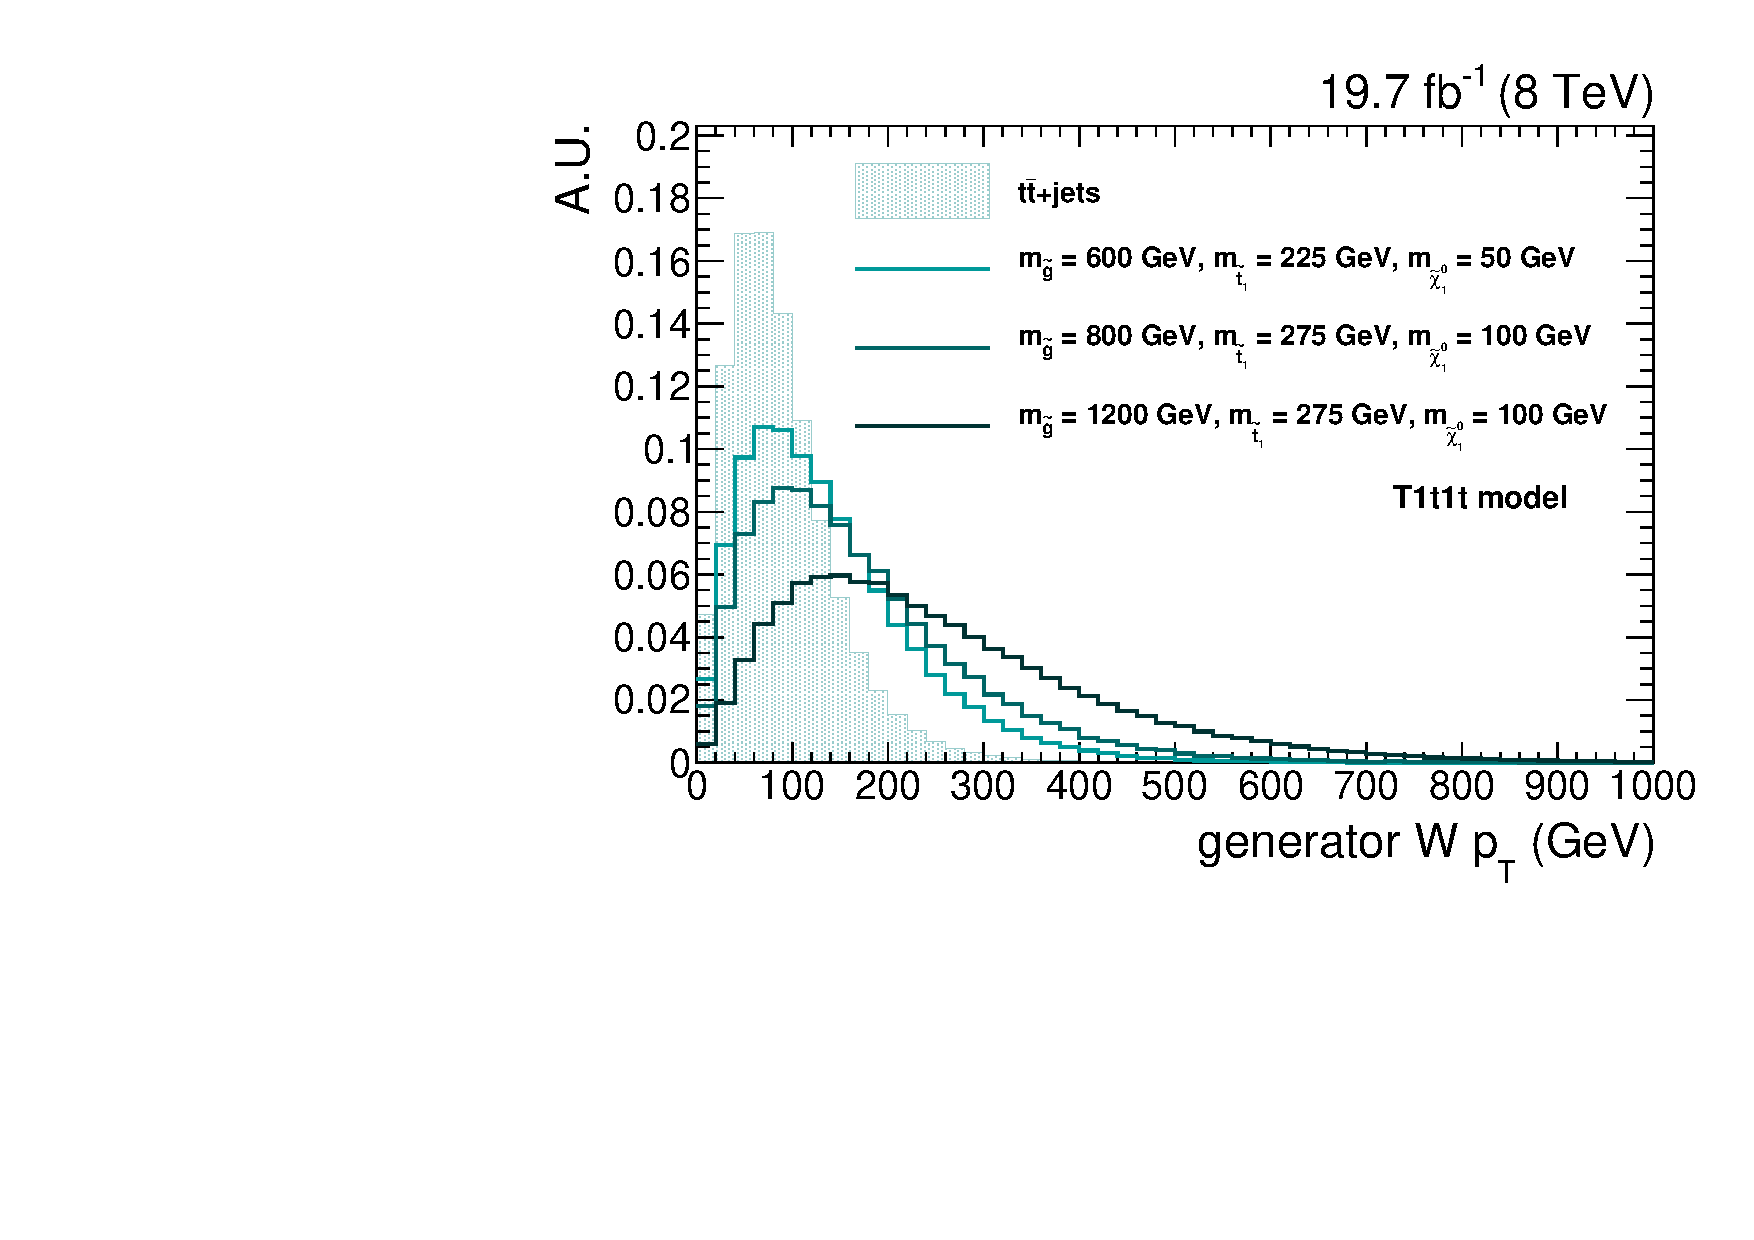
\includegraphics[width=0.48\textwidth]{figures/razor_strategy/T1t1t_genWpt}
\caption{Generator level $\W$ boson \pt for several signal points of the T1ttcc (left) and T1t1t
(right)
simplified models. The average \pt increases as the mass splitting between gluino and top
squark increases. The boost of the $\W$
boson is larger for the signal models considered in comparison to the SM $t\bar{t}$
background. 
The range in \pt needed to have merged decay products for jets with size $\Delta R = 0.5$ is
indicated with an arrow.
\label{fig:boost_gen_Wpt}}
\end{figure}

The razor kinematic variables \mr and \rsq (see Section~\ref{sec:boost_razor} for their
derivation) 
are designed to discriminate processes with new heavy particles and missing energy from Standard
Model processes.
They will be used in this analysis as the main discriminating variables to search for deviations
from the SM. We will perform the search in 25 search bins across the high $\mr$--high $\rsq$ region,
using hadronic events with at least one boosted $\W$ boson and one jet originating from a $\cPqb$
quark (\ie $\cPqb$ jet). 

Standard model backgrounds in the signal regions are estimated using observations in control regions
and global translation factors, calculated from simulated data, that relate the number of events in
one region to that in another. 
Three control regions, $Q$, $W$, and $T$, are defined to select high-purity samples of multijet,
$\W(\rightarrow \ell\nu)+$jets and $t\bar{t}$ processes, respectively.  
The background estimation method uses a likelihood-based approach, with a simultaneous sampling
of systematic uncertainties which fully accounts for any correlations across all bins, backgrounds,
and signals.
%An overview of the different regions and how they are related, including for the control regions
%which background parameters of the likelihood each region constrains, is shown in
%Fig.~\ref{fig:boost_flowchart}. 
The full explanation of the background estimation method will be given in
Section~\ref{sec:boost_likelihood}. 



